% template created by: Russell Haering. arr. Joseph Crop
\documentclass[12pt,letterpaper]{article}
\usepackage{anysize}
\usepackage{cite}
\usepackage{amsmath,amssymb,amsfonts}
\usepackage{algorithm}
\usepackage[noend]{algpseudocode}
\usepackage{graphicx}
\usepackage{multirow}
\usepackage{listings}
\usepackage{xcolor}


\marginsize{2cm}{2cm}{1cm}{1cm}

\lstset{ framexleftmargin=9mm, frame=shadowbox,tabsize = 4}

\begin{document}

\begin{titlepage}
    \vspace*{4cm}
    \begin{flushright}
    {\huge
        ECE 375 Lab 6\\[1cm]
    }
    {\large
    	Timer/Counters
    }
    \end{flushright}
    \begin{flushleft}
    Lab session: 015
    
    Time: 12:00-13:50
    \end{flushleft}
    \begin{flushright}
    Author: Astrid Delestine

    Programming partner: Lucas Plastid 

    \vfill
    \rule{5in}{.5mm}\\
    TA Signature
    \end{flushright}

\end{titlepage}

\section{Introduction}
%This is the first Lab in the ECE 375 series and it covers the setup and compilation of an AVR Assembly Program. The student will learn how how to use the sample Basic Bump Bot assembly file and send the binaries to the AVR Microcontroller board. For the second part of the lab the student will be expected to download and compile the included C sample program and from it learn how to configure the I/O ports of the ATmega32U4 Microcontroller. The student will then write their own C program and upload it to the Microcontroller to verify that it runs as expected. The provided programs have been attached in the source code section of this report.
In this lab the student is expected to learn how to configure the 16 bit Timer/Counter on the ATMEGA32U4 to generate pulse width modulation signals. This is then applied to the LED'S on the bump bot script, to show how speed could be modified on the motors.


\section{Design}
The design for this Lab was created to fulfill the requirements of this lab. External button inputs will be used to increment and decrement the speed at which the PWM signal operates. This is done by offsetting the Timer/Counter 1.

\begin{figure}[h]
	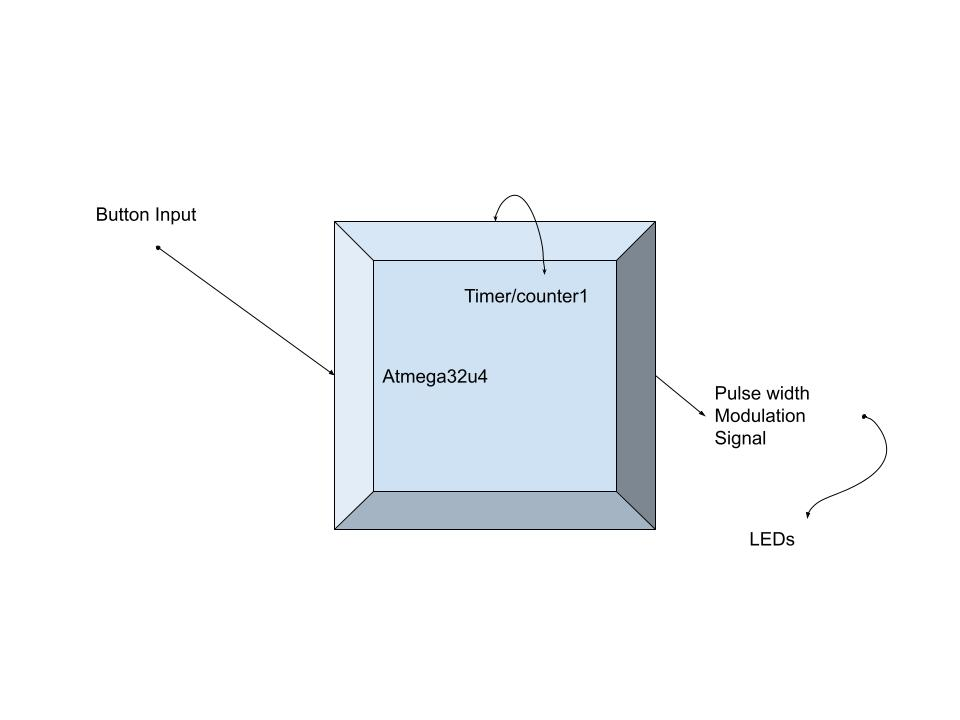
\includegraphics[width=12cm, height=10cm]{Block Diagram L6.jpg}
	\centering
\end{figure}
	
\section{Assembly Overview}
As for the Assembly program an overview can be seen below. 

\subsection{Internal Register Definitions and Constants}
The standard mpr and waitcnt registers are assigned to registers 16 and 17 respectively, as are ilcnt and olcnt to 18 and 19. Additionally a register named speeed is set to r20. This register will control the speed at which out PWM signal operates.

\subsection{Interrupt Vectors}
no interrupt vectors were included in this assignment. 
\subsection{Initialization Routine}
The init routine first setup the stack pointer, then the IO ports B and D are configured fro output and input respectively. Next the 16 bit timer/counter 1 is initialized, this is done through the modification of TCCR1A and TCCR1B. The initial speed is then set by calling the writespd command. Finally the wait counter register is initialized to 100 ms, done by setting it to 5.

\subsection{Main Routine}
The main subroutine just polls the buttons for input, testing to see if any of them are pressed, and if they are, triggering the expected input. This main routine then loops. 


\subsection{Subroutines}
	\subsection{INCSPD}
	This subroutine first checks to see if the max speed has not already been reached, then if not it increments the speed counter. After incrementing the speeed register the WRITESPD subroutine is called. This function will then continue checking to see if the button is being held, and will increment if the button is held, this will handle any bouncing of the button input.
	\subsection{DECSPD}
	This subroutine works the same way that the INCSPD subroutine does, except for the fact that it decrements the speeed register instead of incrementing it.

	\subsubsection{MAXSPD}
	This subroutine sets the max speed for the PWM. To do this it sets the speeed register to 15, the max value. 
	The hold part of the function is then operated, this part fixes any denouncing. 
	 
	
	\subsubsection{WRITESPD}
	The writespd subroutine sets the high byte and the low byte of the speeed register multiplied by 17, this will result in a max value of 255, as the r0 register is moved to mpr. Mpr is then copied to the high and low sides of OCR1A and OCR1B. 
	
	\subsubsection{Wait}
	The standard wait function.
	
	

\section{Testing}
Tested Each button press and compared to external calculations.
\begin{table}[h]
	\centering
	\begin{tabular}{|l|l|l|ll}
		\cline{1-3}
		Case & Expected & Actual meet expected &  &  \\ \cline{1-3}
	d4	&speed increments&	\checkmark  &  \\ \cline{1-3}
	d5	&speed decrements&	\checkmark	&  \\ \cline{1-3}
	d6	&nothing&	\checkmark  &  \\ \cline{1-3}
	d7	&the max speed for the PWM is set&	\checkmark	&  \\ \cline{1-3}
	
%		&          &                      &  &  \\ \cline{1-3}
	\end{tabular}
\caption{Assembly Testing Cases}
\end{table}

\section{Study Questions}
\begin{enumerate}
    \item
    In this lab, you used the Fast PWM mode of 16-bit Timer/Counter, which is only one of many possible ways to implement variable speed on a Tek-Bot. Suppose instead that you used Normal mode, and had it generate an interrupt for every overflow. In the overflow ISR, you manually toggled both Motor Enable pins of the TekBot, and wrote a new value into the Timer/Counter’s register. (If you used the correct sequence of values, you would be manually performing PWM.) Give a detailed assessment (in 1-2 paragraphs) of the advantages and disadvantages of this new approach, in comparison to the PWM approach used in this lab.
    
    Some of the advantages of this approach would be having a more granular understanding and control of the signal, the signal would have to be manually interpreted and whenever it overflows, that overflow would need to be handled. This could be considered either a good thing or a bad thing, however with regards to how this timer was setup in this lab, having more understanding might have been easier to program. While it may be easier to program a more direct approach, using the method taken in this lab results in a clearer end product, in the form of code. In the end however they both function in an externally similar way.
    
    
    \item 
    the previous question outlined a way of using a single 16-bit Timer/Counter in Normal mode to implement variable speed. How would you accomplish the same task (variable TekBot speed) using in CTC mode? Provide a rough-draft sketch of the Timer/Counter-related parts of your design, using either a flow chart or some pseudocode (but not actual assembly code)
    
    \begin{figure}[h]
    	 A drawing of how this might work can be seen below
    	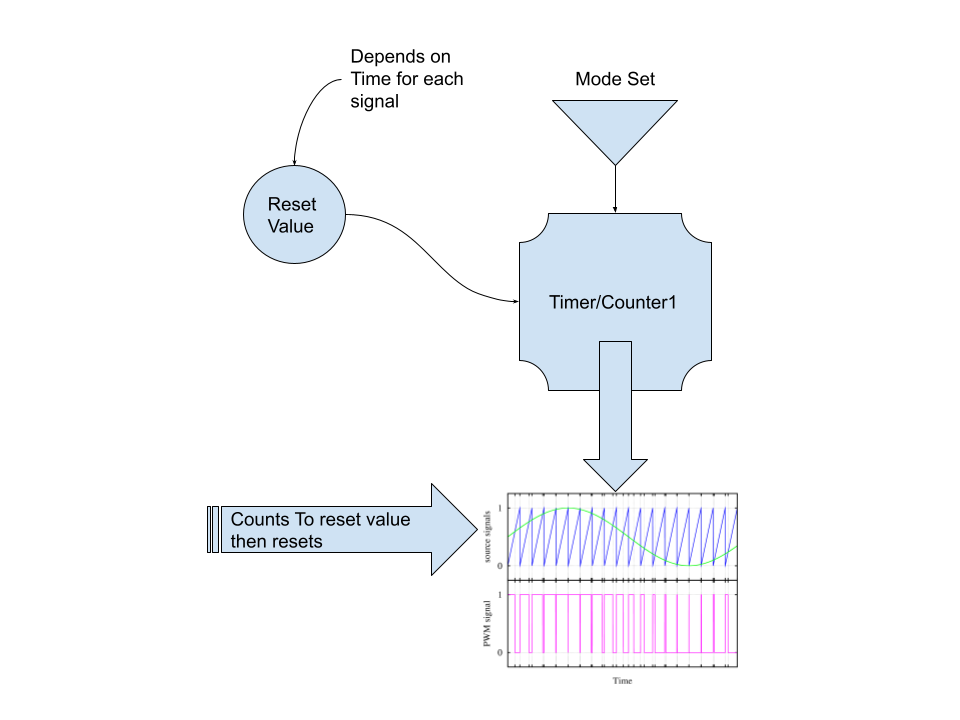
\includegraphics[width=12cm, height=10cm]{q2Drawing.png}
    	\centering
    \end{figure}
   
   
    \item 
	In the next lab, you will be utilizing Timer/Counter1, which can make use of several 16 bit timer registers. The datasheet describes a particular manner in which these registers must be manipulated. To illustrate the process,
	write a snippet of assembly code that configures OCR1A with a value of 0x1234. For the sake of simplicity, you may assume that no interrupts are triggered during your code’s operation.
	
	ldi mpr, High(0x1234) ; You have to set the high first because if you set the low first, you will not actually have set the lower bits correctly.
	sts OCR1AH, mpr
	ldi mpr Low(0x1234)
	sts OCR1AL, mpr
	
    
    \item
    Each ATmega32U4 USART module has two flags used to indicate its current transmitter state: the Data Register Empty (UDRE) flag and Transmit Complete (TXC) flag. What is the difference between these two flags, and which one always gets set first as the transmitter runs? You will probably need to read about the Data Transmission process in the datasheet (including looking at any relevant USART diagrams) to answer this question.
    
    The UDRE flag determines if the USART bus is ready to reccive data. It is set to a 1 when the register of the USART is empty. On the other hand the TXC flag is set when the entire message has been sent. Thus we know that the UDRE flag is set first as the transmitter runs, waiting for the transmit buffer to be empty before loading it with new data.
    
    \item 
    Each ATmega32U4 USART module has one flag used to indicate its current receiver state (not including the error flags). For USART1 specifically, what is the name of this flag, and what is the interrupt vector address for the
    interrupt associated with this flag? This time, you will probably need to read about Data Reception in the datasheet to answer this question
    
    The name of the flag for USART1 is UDRE1, and its interrupt vector location is \$0034 
    
       
    
\end{enumerate}

\section{Difficulties}
This Lab was only diffucult due to the fact that there was a lot of reading and direct understanding of the AVR manual. Besides that the lab was quite simple to understand.

\section{Conclusion}
In conclusion, this lab allowed the student to experiment with using the 16 bit timer/counter and gain a better understanding for how dimming LEDs work and how motor speed control can work. Additionally the student learned how to find specific item in the AVR manual in a faster and clearer way. While this may not have been an intended goal of the lab, it was a useful outcome.

\pagebreak

\section{Source Code}%
\lstinputlisting
[
caption=Assembely Script,
language={[x86masm]Assembler},
numbers =left,
rulesepcolor=\color{blue}
]{../Lab6Assm/Lab6Assm/Astrid_Delestine_and_Lucas_Plaisted_Lab6_sourcecode.asm}





\end{document}